\newpage
\section*{Метод распределенной трассировки лучей} 

Рассмотренные выше подходы в рамках трассировки лучей можно использовать для расчета сложных материалов с неоднозанчным поведением. Пуская лучи в нескольких разных направлениях получаем возможность моделировать поверхности с произвольной функцией ДФО \cite{ray-tracing}.

Данный подход увеличивает количество испускаемых лучей, а значит вычислительная сложность возрастает по сравнению с вышеприведенными алгоритмами обычной трассировки. Такова цена за универсальность двулучевой функции отражения. 

\begin{center}
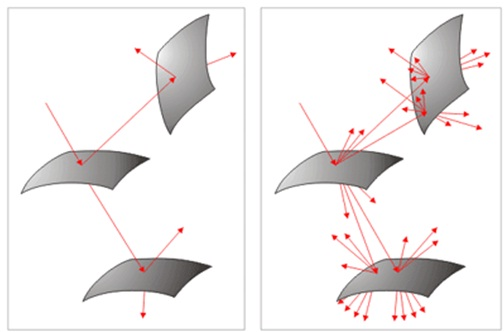
\includegraphics[width=0.7\linewidth]{ray-tracing-wide.jpg}
\end{center}

Основу этого алгоритма мы и изберем для реализации нашей программы